\documentclass[a4paper, 12pt, oneside]{book}
\usepackage{graphicx}
\usepackage[french]{babel}
\usepackage[utf8]{inputenc}
\usepackage[T1]{fontenc}
\frenchbsetup{StandardLists=true}
\usepackage{enumitem}
\usepackage{multirow}
\usepackage{listings}
\usepackage{float}
\usepackage{hyperref}
\usepackage{url}
\usepackage[french]{algorithm}
\usepackage{style/myalgorithm}
\usepackage{amsmath,amsfonts,amssymb}
\newcommand{\fBm}{\emph{fBm}~}
\newcommand{\etal}{\emph{et al.}~}
\newcommand{\glAd}{\emph{GL4D}~}
\newcommand{\apiopengl}{API OpenGL\textsuperscript{\textregistered}~}
\newcommand{\opengl}{OpenGL\textsuperscript{\textregistered}~}
\newcommand{\opengles}{OpenGL\textsuperscript{\textregistered}ES~}
\newcommand{\clang}{langage \texttt{C}}
\newcommand{\codesource}{\textsc{Code source}~}
\floatstyle{ruled}
\newfloat{programslist}{htbp}{locs}
\newcommand{\listofprograms}{\listof{programslist}{Liste des codes source}}
\newcounter{program}[subsection]
\renewcommand{\theprogram}{\arabic{chapter}.\arabic{program}}

\newenvironment{program}[1]{
  \if\relax\detokenize{#1}\relax
  \gdef\mycaption{\relax}
  \else
  \gdef\mycaption{#1}
  \fi
  \refstepcounter{program}
  \addcontentsline{locs}{section}{#1}
  \footnotesize
}{
  \begin{description}
    \item[\codesource \theprogram]--~\mycaption
  \end{description}
}

\begin{document}
\begin{titlepage}
  \begin{center}
    \begin{tabular*}{\textwidth}{l@{\extracolsep{\fill}}r}
      
\includegraphics[height=1.5cm]{images/m1info.png}&
      
\includegraphics[height=1.5cm]{images/oaccueil.png}
    \end{tabular*}
    \small 
    \rule{\textwidth}{.5pt}~\\
    \large 
    \textsc{Université Paris 8 - Vincennes à Saint-Denis}\vspace{0.5cm}\\
    \textbf{M1 MIASHS : Big Data et fouille de données}\vspace{3.0cm}\\
    \Large
    \textbf{Création d'une architecture distribuée et analyse de données}\vspace{1.5cm}\\
    \large
    \textbf{PANCHALINGAMOORTHY \textsc{Gajenthran}}\vspace{1.5cm}\\
  \end{center}\vspace{1.5cm}~\\
  \begin{tabular}{ll}
    \hspace{-0.45cm}Organisme d'accueil~:~&~Université Paris 8\\
    \hspace{-0.45cm}Cours ~:~&~Cadre logiciel pour le Big Data\\
  \end{tabular}
\end{titlepage}
\frontmatter

%% Table des matières
\tableofcontents
\mainmatter

%% Introduction
\chapter[Introduction]{Introduction}
Avec l'emergence des entreprises de streaming, les utilisateurs consomment de plus de plus de films, de séries ou encore d'oeuvres cinématographiques. La satisfaction des utilisateurs représente donc un enjeu important pour les entreprises telles que Netflix, Amazon Prime ou encore Disney+. Cela passe donc par un système de recommendation de films afin d'avoir un gain de temps conséquent et d'améliorer l'expérience utilisateur.
\newline
A l'aide de l'architecture distribuée \texttt{Amazon Web Services} (AWS), nous nous pencherons sur ce sujet et analyserons les données à l'aide d'\texttt{Hive}. Apache Hive est une infrastructure d’entrepôt de données intégrée sur Hadoop permettant l'analyse, le requétage via un langage proche syntaxiquement de SQL ainsi que la synthèse de données. Bien que initialement développée par Facebook, Apache Hive est maintenant utilisée et développée par d'autres sociétés comme Netflix. Amazon maintient un fork d'Apache Hive qui inclut Amazon Elastic MapReduce dans Amazon Web Services (source: Wikipédia).
\newline
Dans ce papier, nous allons d'abord décrire les datasets utilisées pour la phase d'analyse, puis nous créerons l'architecture distribuée AWS, puis nous détaillerons les différents requêtes \texttt{Hive}, ensuite nous comparerons l'efficacité de ce dernier avec un autre langage et enfin nous discuterons à propos des avantages proposés par l'architecture distribuée.

\chapter[Datasets]{Datasets}
Le système de recommendation se reposera quasiment que sur les films. Afin d'obtenir des résultats fiables et de profiter pleinement de l'architecture distribuée, une base de données d'environ 1Go a été récupérée, en format \textit{.csv}. Elle a été repris de \textit{Kaggle} qui elle-même vient des films listés par \textit{MovieLens}, et contient des films venant de 2018 ou avant. Celle-ci est découpée en plusieurs parties:
\begin{itemize}
	\item \textit{movies.csv}: regroupe l'identifiant des films (\texttt{movieId}), l'identifiant des films sur le site IMDB (\texttt{imdb\_id}) et le titre des films (\texttt{title}).
	\item \textit{ratings.csv}: regroupe l'identifiant des utilisateurs (\texttt{userId}), l'identifiant des films (\texttt{movieId}), et la note des utilisateurs (\texttt{rating}) sur 5 et la date à laquelle ils ont noté (\texttt{timestamp}).
	\item \textit{votes.csv}: regroupe l'identifiant des utilisateurs (\texttt{userId}), l'identifiant des films (\texttt{movieId}), l'identifiant des films sur le site IMDB (\texttt{imdb\_id}) et le vote moyen des films (\texttt{vote\_average}) et le nombre de votant pour chaque film (\texttt{vote\_count}).
\end{itemize}

Ainsi, nous nous appuyons sur une base de données de plus de 45K films et notamment 26 millions de votes dont plus de 250K votants.

\chapter[AWS]{Création d'une architecture distribuée (AWS)}
Suite à la limite de crédit dépassé sur le compte, le projet a donc du être reporté sur un autre compte mais cela n'aura une influence ni sur le fonctionnement de l'architecture, ni sur les explications apportées ci-dessous.
\newline 
Afin de bénéficier des services proposés par AWS, il fallait tout d'abord se connecter à celui-ci. Pour cela, nous sommes passé par l'interface \texttt{RosettaHUB} (fig.\ref{fig:rosettahub}) afin de créer de notre compte (déjà réalisé lors des séances "Cadre logiciel pour le Big Data"). Une fois le compte créé, nous devons alimenter notre compte en crédit pour pouvoir utiliser les services AWS. Les détails seront épargnés vu qu'il s'agit ici de manoeuvres déjà exécutées en cours.
\newline
Dès que les prépartifis sont terminés, nous pouvons nous attaquer à l'architecture. Tout d'abord, nous devons créer une instance en se dirigeant vers le service \texttt{EC2}. Un tutoriel a été mis en ligne sur la plateforme Moodle afin d'expliquer en détails les différentes étapes à suivre pour lancer une instance. 
\newline
Avant de nous occuper des clusters, nous allons dans un premier temps, récolter les données depuis notre ordinateur et les placer dans le service S3. 

\begin{figure}[H]
  \centering
  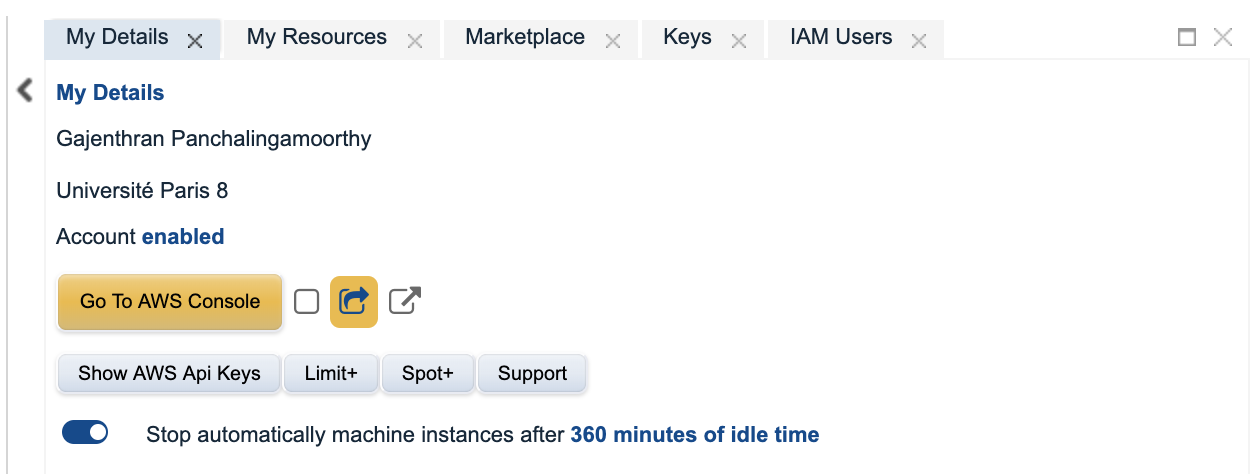
\includegraphics[width=1.0\textwidth]{images/rosettahub}
  \caption{Interface \texttt{RosettaHUB}}
  \label{fig:rosettahub}
\end{figure}

\section{Service S3}
Le service S3 permet de stocker les données en ligne dans le cloud afin qu'on puisse les réutiliser avec d'autres services d'AWS dans la section suivante. Il offre la possibilité de stocker n'importe quelle quantité de données et également d'assurer leurs protections avec une sécurité très fiable. Pour profiter de ce service, dirigeons nous vers la console AWS, et cherchons le service \texttt{S3}.
\newline
Le service \texttt{S3} range les données par compartiments (fig.\ref{fig:s3-home}). Pour ajouter de nouvelles données, il suffit de créer un compartiment en cliquant sur le bouton \textit{Créer un compartiment}. Cela ouvrira une nouvelle fenêtre dans laquelle nous préciserons le nom du compartiment pour pouvoir l'identifier et le récupérer lors de notre connexion (fig.\ref{fig:s3-compartiment}). Une fois le compartiment créé, nous pouvons importer des fichiers à travers le bouton \textit{Charger} et de charger les fichiers que nous souhaitons. Les fichiers sont plutôt lourds donc le temps des transactions risque de durer assez longtemps. A noter que ne nous comptons pas utiliser toutes les données de la base de données, donc une répartition des données de façon judicieuse s'impose \footnote{Toutes les colonnes des fichiers \textit{.csv} ne vont pas être exploitées, ainsi la décision de supprimer les colonnes inutiles a été prise afin d'alléger la taille de la base.}. De plus, afin d'avoir une base de données plus organisées, nous pouvons également les ranger dans des dossier avec \textit{Créer un dossier}.

\begin{figure}[H]
  \centering
  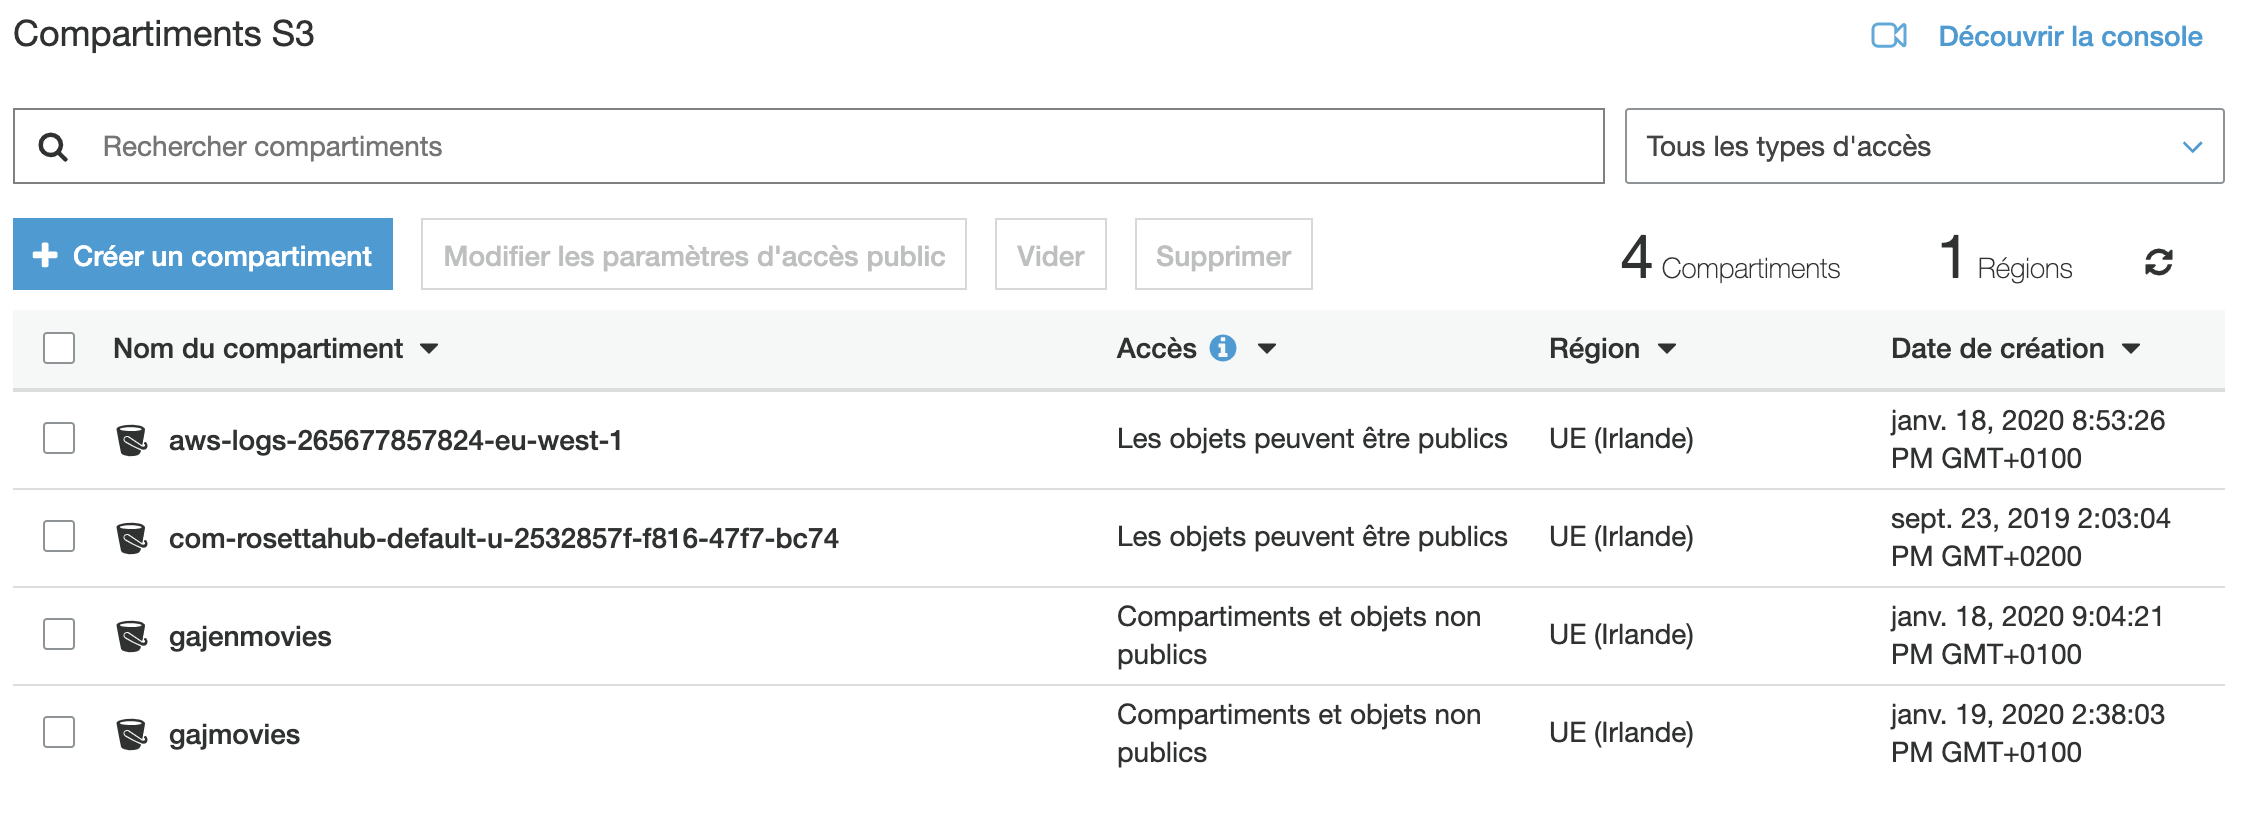
\includegraphics[width=1.0\textwidth]{images/s3-home}
  \caption{Amazon \texttt{S3} et son rangement par compartiment}
  \label{fig:s3-home}
\end{figure}

\begin{figure}[H]
  \centering
  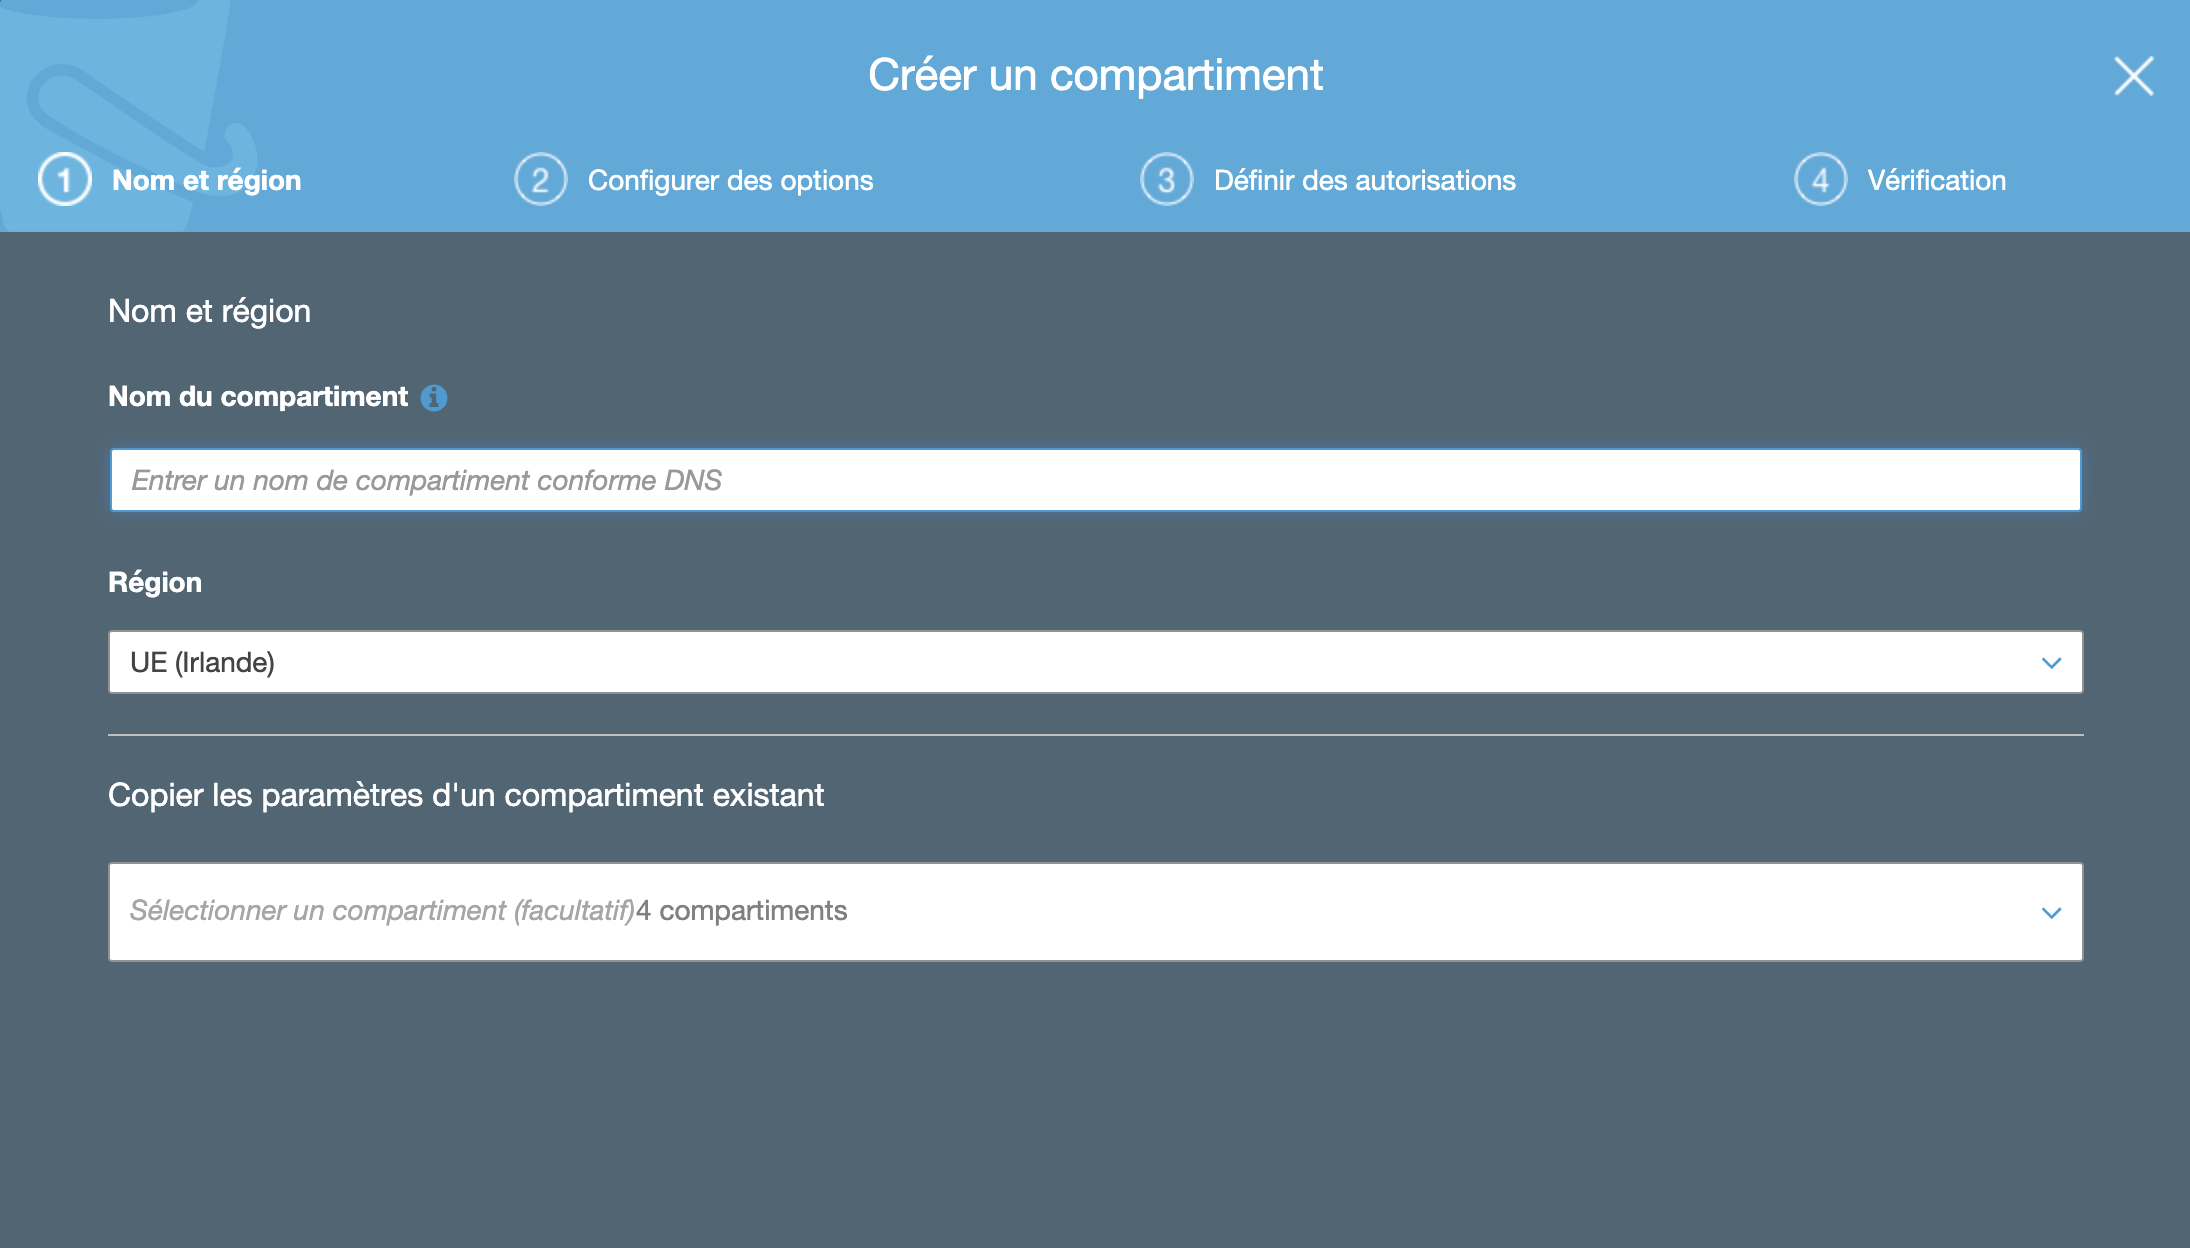
\includegraphics[width=1.0\textwidth]{images/s3-compartiment}
  \caption{Création d'un nouveau compartiment dans Amazon \texttt{S3}}
  \label{fig:s3-compartiment}
\end{figure}


\section{Service EMR}
Désormais, nous pouvons lancer les clusters. Pour cela, nous allons nous rediriger vers la console AWS et chercher le service \texttt{EMR}. Le service \texttt{EMR} (fig.\ref{fig:emr-home}) est la plateforme de mégadonnées native cloud leader qui traite de grandes quantités de données rapidement et à moindre coût. Utilisant des outils open source tels que \texttt{Apache Spark}, \texttt{Apache Hive}, \texttt{Apache HBase}, \texttt{Apache Flink}, \texttt{Apache Hudi} (Incubating) et \texttt{Presto}, associés à la scalabilité dynamique d'Amazon \texttt{EC2} et au stockage évolutif d'Amazon \texttt{S3} (source: AWS.Amazon.com).

\begin{figure}[H]
  \centering
  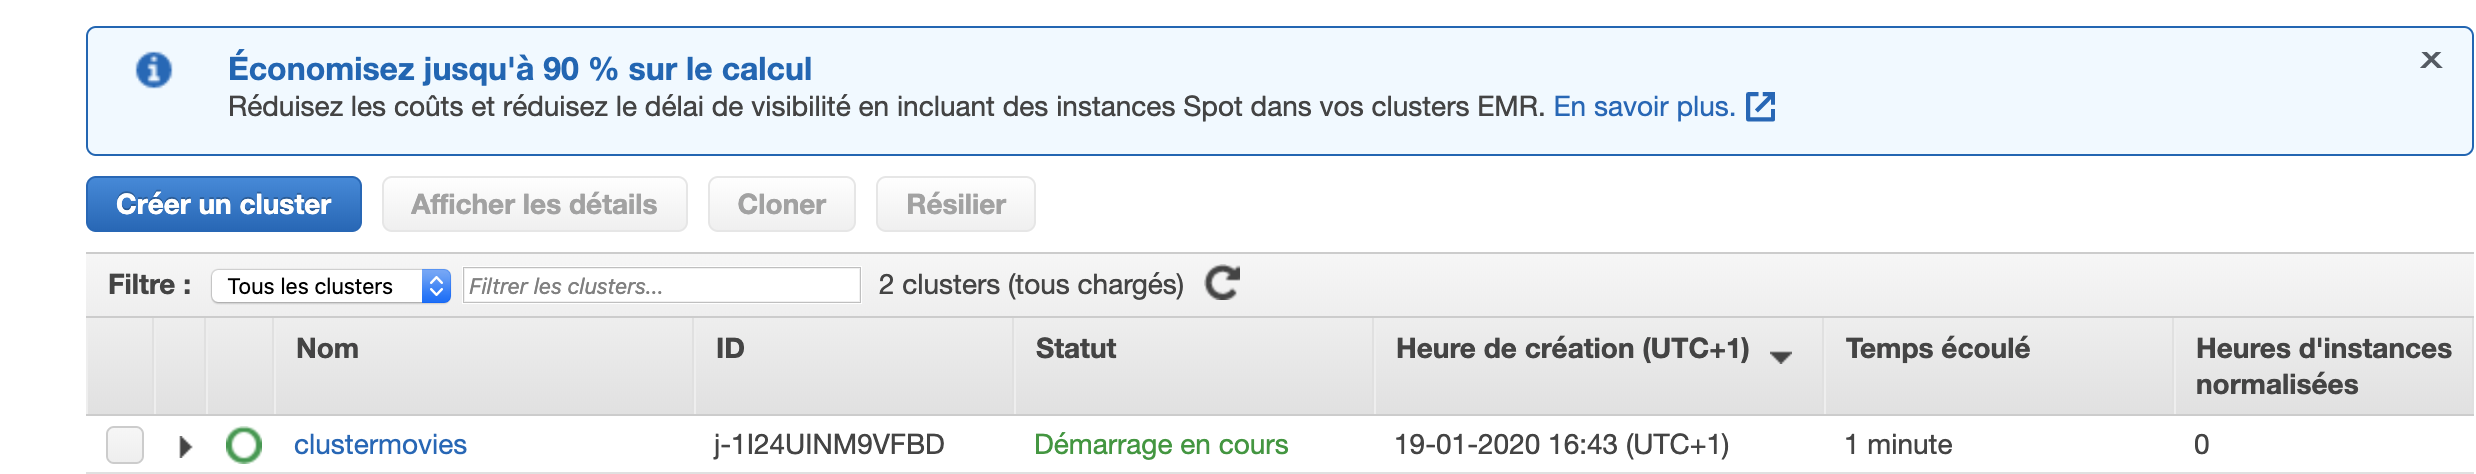
\includegraphics[width=1.0\textwidth]{images/emr-home}
  \caption{Amazon EMR et la liste des clusters}
  \label{fig:emr-home}
\end{figure}

En cliquant sur \textit{Créer un cluster}, nous allons pouvoir créer un nouveau cluster (fig.\ref{fig:emr-create}). Il y a plusieurs paramètres à remplir comme le nom du cluster, les logiciels pouvant être utilisés (en l'occurence, pour ce projet, Coore Hadoop sera utilisé). 

\begin{figure}[H]
  \centering
  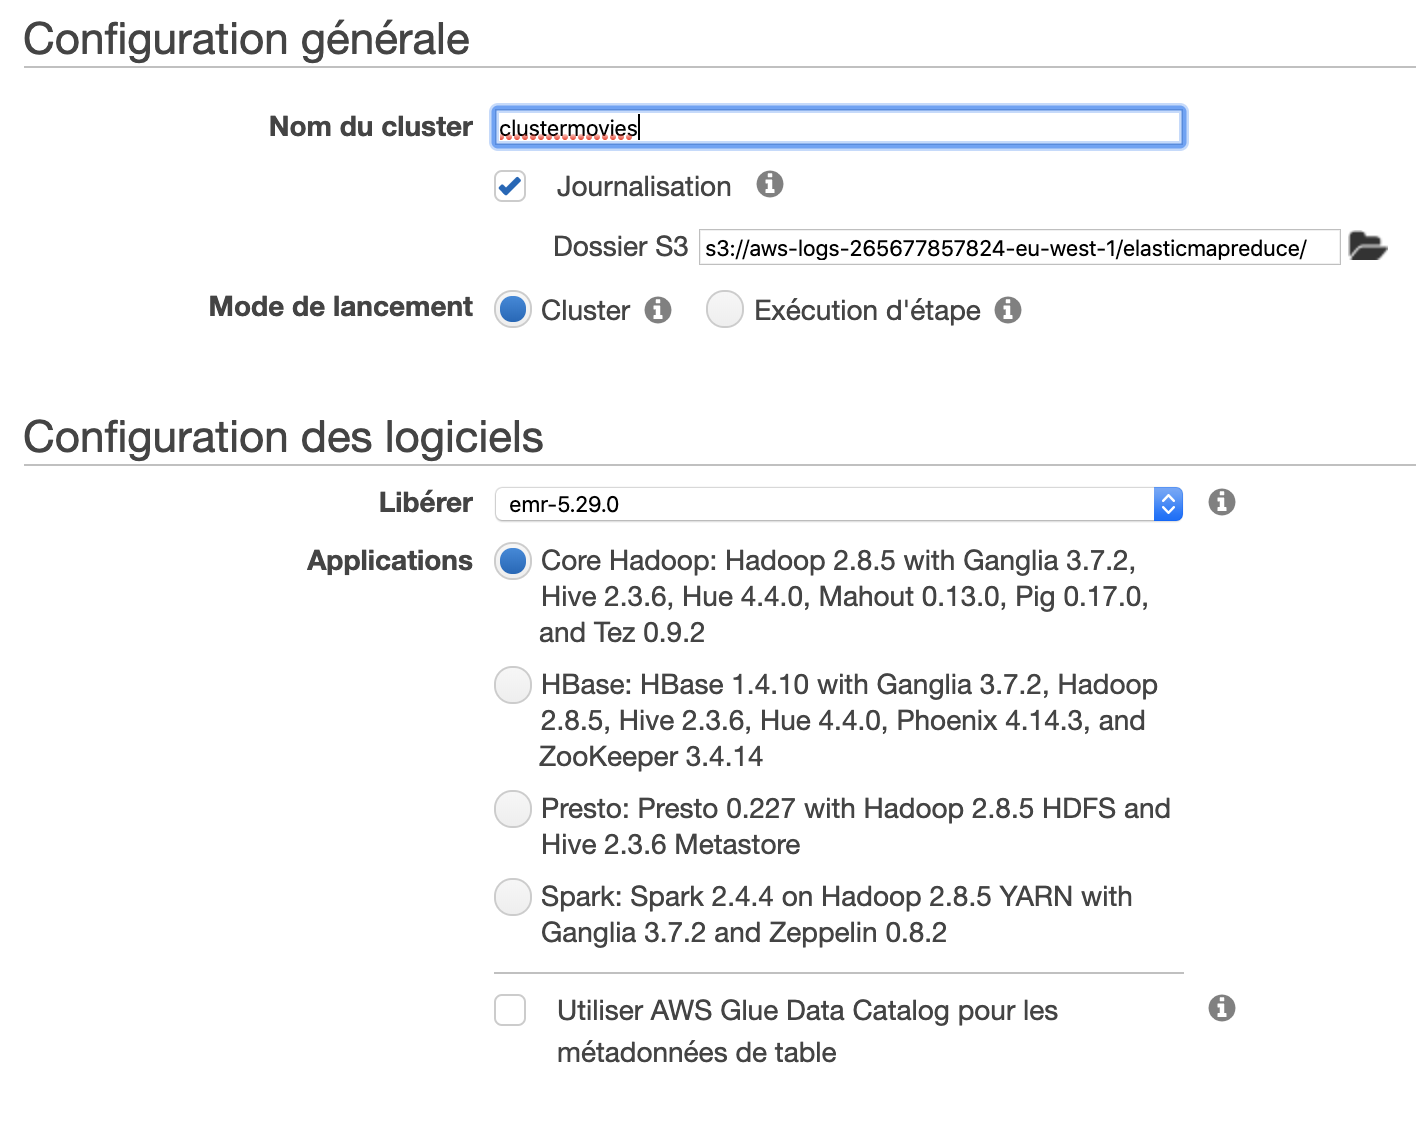
\includegraphics[width=1.0\textwidth]{images/emr-create}
  \caption{Création de clusters dans Amazon \texttt{EMR}} 
  \label{fig:emr-create}
\end{figure}

De plus, nous préciserons le nom de la clé que nous avons instancié, avec comme nombre équivalent d'instance à 3 (à savoir 1 noeud maître et 2 noeuds principaux) avec le type d'instance \textit{m3.xlarge} afin d'éviter la surconsommation (fig.\ref{fig:emr-cle})

\begin{figure}[H]
  \centering
  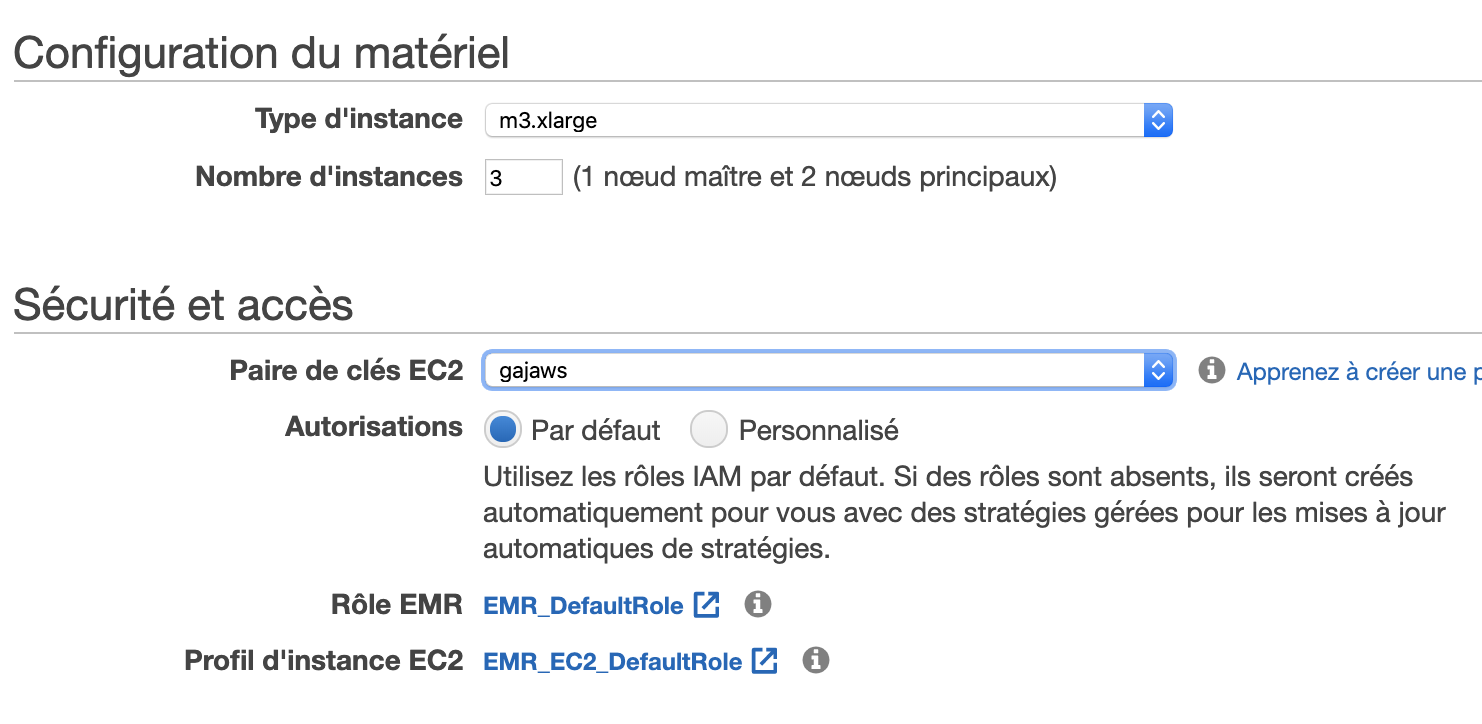
\includegraphics[width=1.0\textwidth]{images/emr-cle}
  \caption{Choix des instances dans Amazon \texttt{EMR}}
  \label{fig:emr-cle}
\end{figure}

Puis, pour établir la connexion ssh et profiter des fonctionnalités proposées par \texttt{EMR}, attendez que votre soit totalement prêt (symbolisé par un rond rempli en vert), puis dirigez vous sur le cluster en question afin de trouver la commande utile à la connexion (fig.\ref{fig:terminal-connexion}). 

\begin{figure}[H]
  \centering
  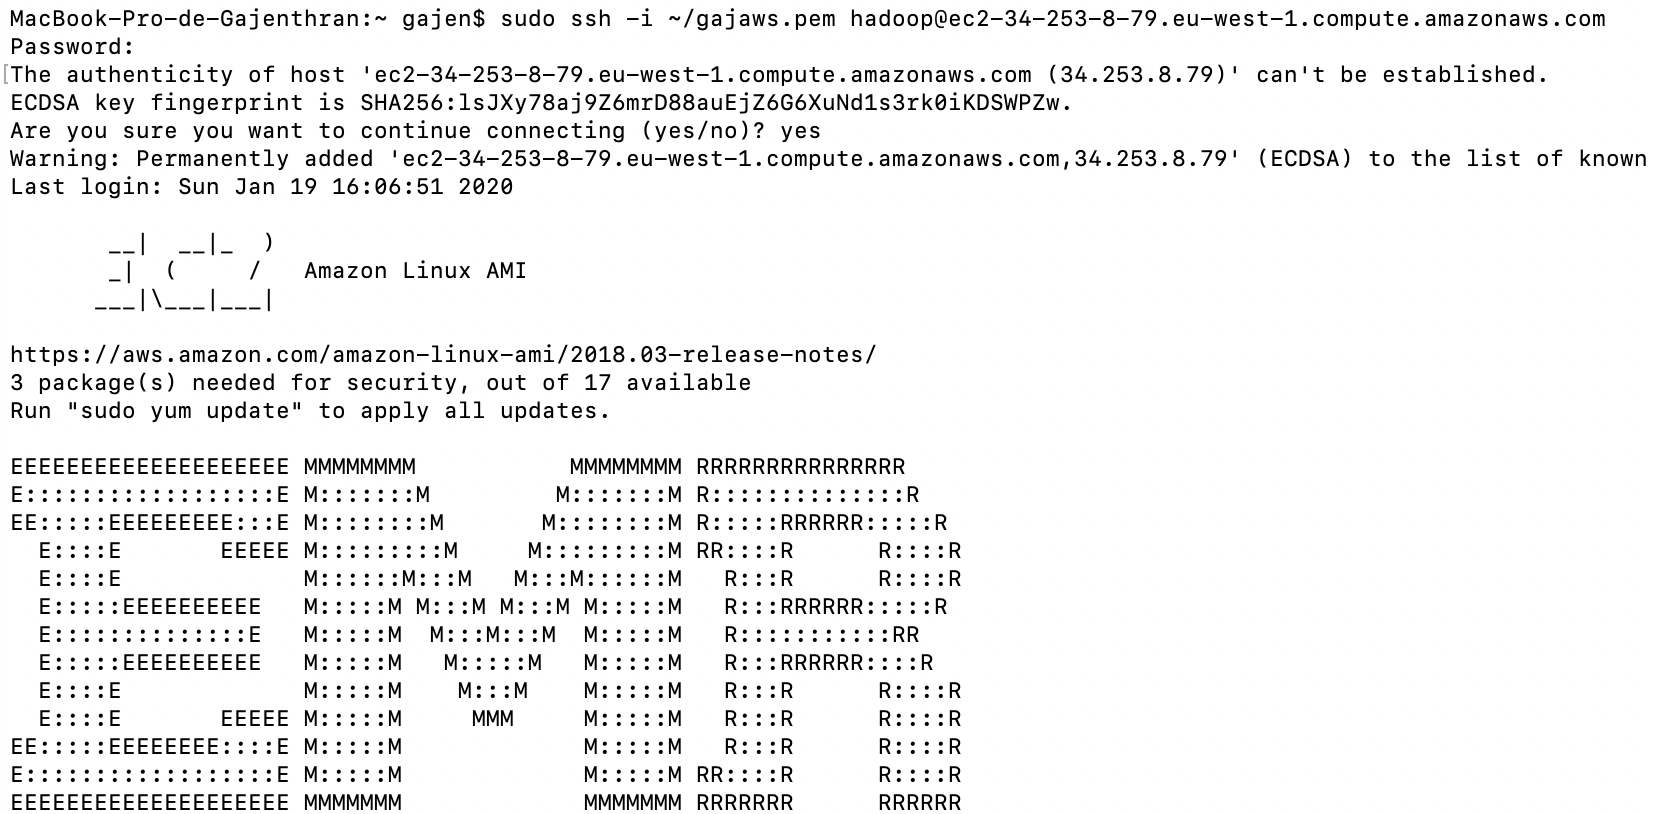
\includegraphics[width=1.0\textwidth]{images/terminal-connexion}
  \caption{Etablissement de la connexion ssh avec \texttt{EMR}}
  \label{fig:terminal-connexion}
\end{figure}

La connexion étant établie, il nous reste à transférer les fichiers stockés dans \texttt{S3} (fig.\ref{fig:terminal-s3}, dans notre \texttt{EMR} à l'aide de l'argument \texttt{-copyToLocal} en indiquant le nom de notre compartiement (fig.\ref{fig:terminal-toLocal}. Une fois les fichiers \textit{.csv} importés localement, il faudra envoyer ces fichiers dans \texttt{/user/hadoop/} via l'argument \texttt{-fromLocal} (fig.\ref{fig:terminal-fromLocal}).

\begin{figure}[H]
  \centering
  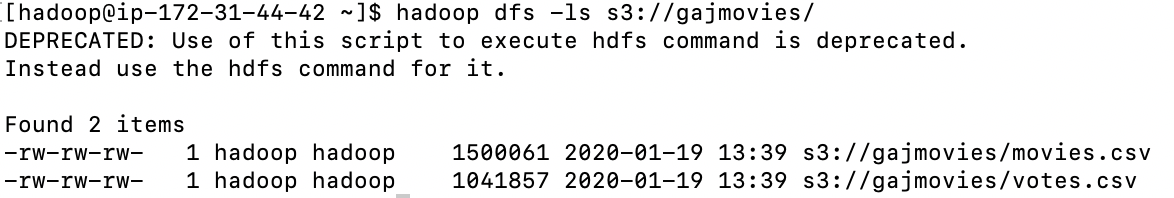
\includegraphics[width=1.0\textwidth]{images/terminal-s3}
  \caption{Affichage des compartiments stockés sur \texttt{S3} avec \texttt{EMR}}
  \label{fig:terminal-s3}
\end{figure}

\begin{figure}[H]
  \centering
  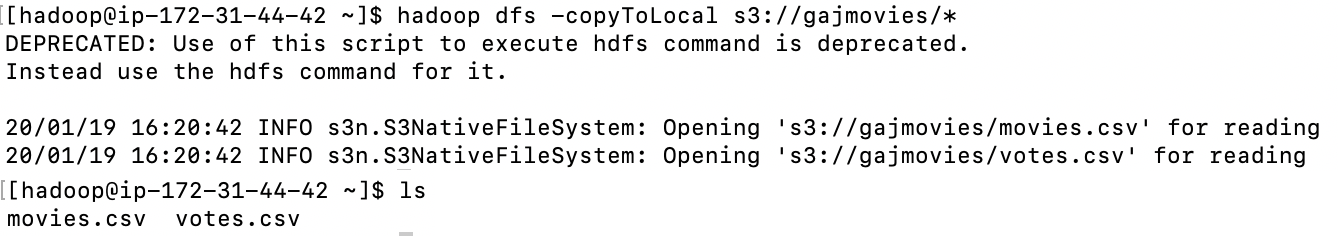
\includegraphics[width=1.0\textwidth]{images/terminal-toLocal}
  \caption{Copie des fichiers contenus dans \texttt{S3} avec \texttt{EMR}}
  \label{fig:terminal-toLocal}
\end{figure}

\begin{figure}[H]
  \centering
  
\includegraphics[width=1.0\textwidth]{images/terminal-fromLocal}
  \caption{Transfert des fichiers locaux dans \texttt{/user/hadoop/} avec \texttt{EMR}}
  \label{fig:terminal-fromLocal}
\end{figure}

Désormais, il nous reste plus qu'à exploiter \texttt{Hive} afin d'analyser les données que nous venons de récupérer. Pour tester si le logiciel fonctionne correctement, il suffit de taper la commande \texttt{hive}, ou \texttt{hive -f <fichier.hive>}.

\chapter{Analyse des données (Hive)}
Pour l'analyse de données, comme nous l'avons dit, nous nous focaliserons sur le langage \texttt{Hive}. Le système de recommendation d'un film peut prendre plusieurs formes, il peut être simple comme assez complexe. Il peut se baser sur les notes, sur le contenu d'un film, sur les goûts de l'utilisateur...

\section{Initialisation des tables}
Avant toute chose, commençons par créer les tables à partir de la base de données. Les créations des tables se trouveront dans \textit{init\_rs.hive}. À l'aide de \texttt{CREATE EXTERNAL TABLE IF NOT EXISTS} (fig.\ref{fig:hive-init}) pour créer une table, nous préciserons le même nombre de colonne que les fichiers \textit{.csv}. D'ailleurs, nous préciserons à la fin de l'instruction que les tuples des fichiers \textit{.csv} sont délimités par des virgules comme suit \texttt{ROW FORMAT DELIMITED FIELDS TERMINATED BY ',';}. Les types que nous utiliserons principalement concerneront les entiers \texttt{INT}, les chaînes de caractères \texttt{STRING}, les flottants \texttt{FLOAT}. 
\newline
Nous tenons également à mentionner l'ajout de la partition sur l'année de sortie des films qui va avoir un rôle déterminant vu qu'il s'agit de films repris des années 2017 principalement. Pour récupérer les fichiers \textit{.csv} de \texttt{/user/hadoop/}, \texttt{LOAD DATA INPATH <path> INTO TABLE <table>;} se chargera de mettre en place les table pour pouvoir exploiter la base de données.

\begin{figure}[H]
  \centering
  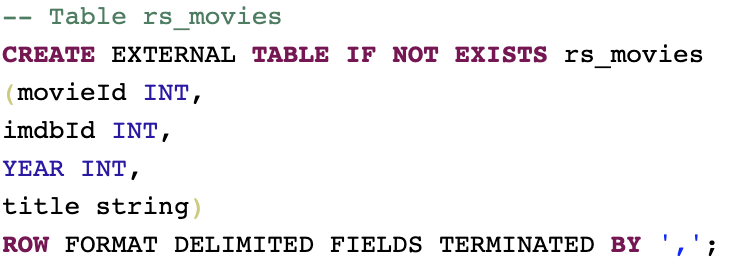
\includegraphics[width=1.0\textwidth]{images/hive-init}
  \caption{Création des tables sur \texttt{Hive}}
  \label{fig:hive-init}
\end{figure}

\section[Hive]{Système de recommendation}
Plusieurs systèmes de recommendation seront étudiés afin de tester l'efficacité que cela soit en terme de temps ou encore de la pertinence des résultats obtenus.
\subsection{Simple système de recommendation}
Un simple système de recommendation qui se base uniquement sur les votes moyens des utilisateurs d'un film. Nous nous contentons de classer par ordre décroissant les votes des films et établir une liste des films les plus populaires de cette manière (fig.\ref{fig:hive-popular}). 
\newline
Pour cela, nous devons réaliser une jointure entre les tables \texttt{rs\_movies} et \texttt{vote} afin de mélanger les colonnes \texttt{titre} et \texttt{vote\_average}. La jointure se reposera sur la clé \texttt{movieId} (des deux côtés). Pour ranger les enregistrements par ordre décroissant, \texttt{ORDER BY ... DESC} nous sera utile. Pour finir, on affichera seulement les 5 films les plus populaire avec \texttt{LIMIT 5}.

\begin{figure}[H]
  \centering
  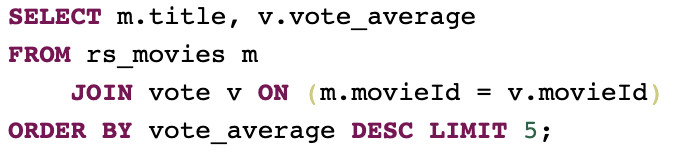
\includegraphics[width=1.0\textwidth]{images/hive-popular}
  \caption{Requête pour un simple système de recommendation}
  \label{fig:hive-popular}
\end{figure}

\subsection{Système de recommendation basé sur une note mesurée}
Pour obtenir un système plus fiable, nous allons effectuer quelques ajustements au premier système. Tout d'abord, pour obtenir des résultats optimaux, les films n'ayant pas dépassé un certain seuil de vote $ \tau $ ne pourront pas faire partis de cette liste. Ensuite, nous ajouterons à la table \texttt{vote}, une nouvelle colonne \texttt{wr} qui représentera une note mesurée qui se réfère à la formule suivante: $ (\frac{vc}{vc + \tau} * avg) + (\frac{\tau}{\tau + vc} * \mu) $ où \textit{vc} correspond à nombre de vote d'un film, \textit{avg} à la note moyenne d'un film, $ \tau $ au seuil minimal pour accepter un film et $ \mu $ au vote moyen des films. Une fois toutes les lignes de la colonne \texttt{wr} remplies, nous choisirons les 5 premiers films.
Pour cela, \texttt{ALTER TABLE ... ADD COLUMNS} ajoutera une nouvelle colonne \texttt{wr} sur la table \texttt{vote}. Nous calculerons $ \mu $ et $ \tau $ et les stockeront respectivement dans les variables \texttt{avg\_votes} et \texttt{vote\_counts} en utilisant la fonction \texttt{percentile}. En ajoutant la colonne, il nous reste simplement à remplir chaque case avec \texttt{UPDATE ... SET} de la colonne grâce la formule vue précédemment. Les variables initialisées au départ seront exploitées à l'aide de la notation suivante: \texttt{\${hiveconf:<variable>}}. Désormais, il nous suffit de retirer de la table les enregistrements ayant les plus grandes valeurs \texttt{wr}.

\begin{figure}[H]
  \centering
  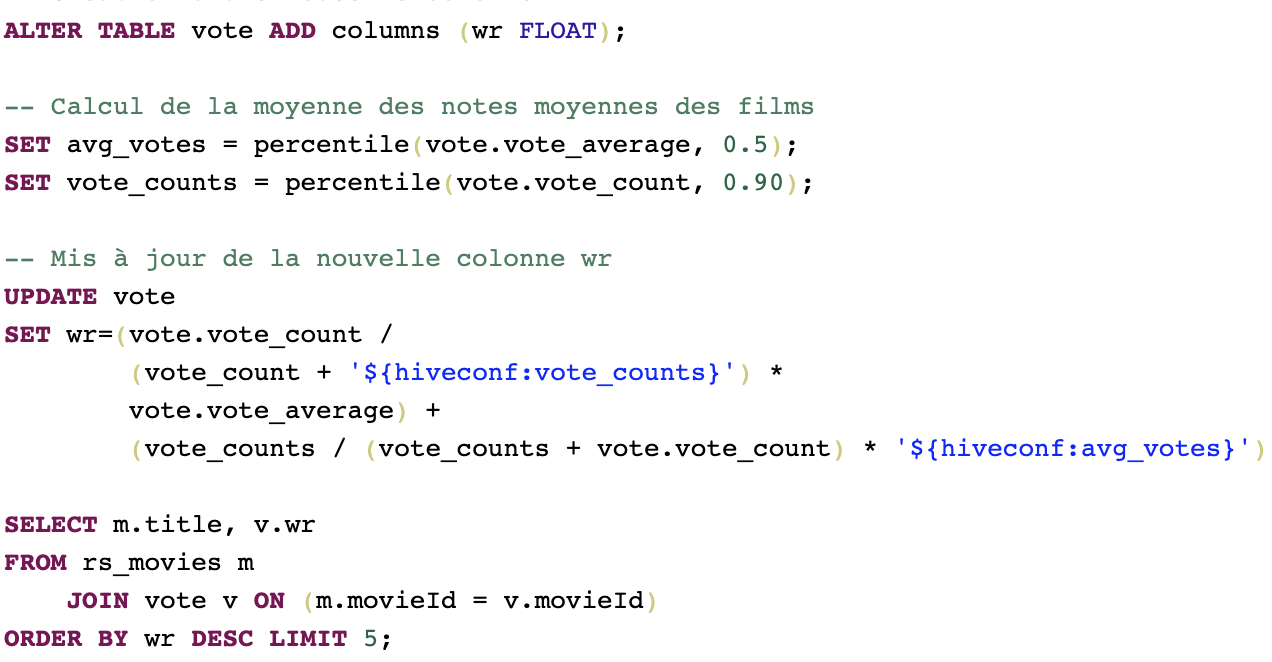
\includegraphics[width=1.0\textwidth]{images/hive-wr}
  \caption{Requête pour un système de recommendation plus sophistiqué}
  \label{fig:hive-wr}
\end{figure}

\subsection{Système de recommendation basé sur la catégorie}
Par ailleurs, il est également possible de renforcer le système actuel par un filtrage concernant le genre des films (fig.\ref{fig:hive-categorie}). En effet, il est légèrement compliqué de parser un objet JSON via \texttt{Hive} mais il est possible de contourner le problème d'une manière différente. Cela nécessite, dans un premier lieu, la jointure de 3 tables \texttt{vote}, \texttt{rs\_movies} et \texttt{genres} en utilisant des \texttt{JOIN}. Dès que les liaisons faites, il faudra filtrer les tuples en se basant sur la colonne \texttt{genres}. La condition \texttt{g.genres LIKE '\%Romance\%'} fera l'affaire pour conserver seulement les films romantiques dans notre table. Nous essayerons pas de parser les objets afin de distinguer les différents genres d'un film, nous nous contenterons de vérifier si l'objet (considéré comme une chaîne de caractère) contient le mot demandé (en l'occurence "Romance" dans notre cas).

\begin{figure}[H]
  \centering
  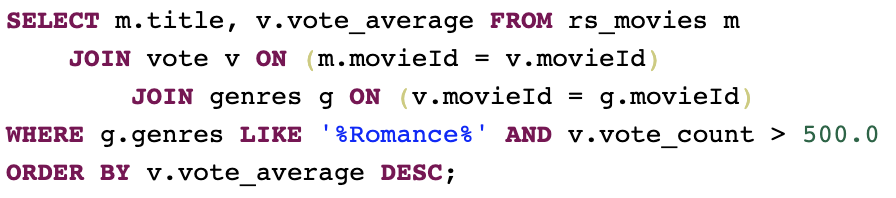
\includegraphics[width=1.0\textwidth]{images/hive-categorie}
  \caption{Requête pour un système de recommendation ajoutant les genres}
  \label{fig:hive-categorie}
\end{figure}

\chapter{Comparaison de Hive et Python}
Pour comparer l'importance des clusters et d'\texttt{Hive}, nous allons comparer les résultats obtenus lors de la réalisation de \texttt{Python}. Le fichier \textit{MR\_Popular.py} contient plus ou moins la même fonctionnalité proposées par le système plus sophistiqué d'\texttt{Hive} avec une note mesurée (fig.\ref{fig:python-wr}). 
\newline
Si nous comparons en termes de code les deux systèmes, il y a très peu de différence que l'on peut remarquer (fig.\ref{fig:python-hive})). La différence se manifeste surtout au niveau de l'exécution des tâches et du temps consacré. \texttt{Hive} semble avoir une longueur d'avance notamment grâce à \texttt{EMR} qui le rend plus efficace.
% \chapter{Conclusion}

\begin{figure}[H]
  \centering
  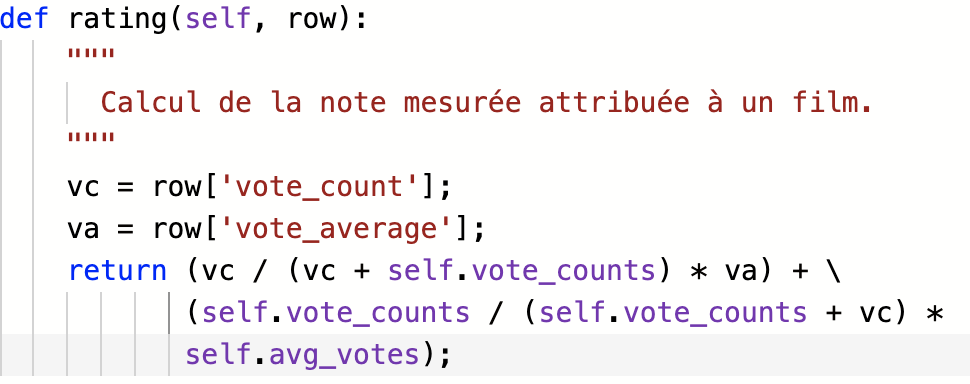
\includegraphics[width=1.0\textwidth]{images/python-wr}
  \caption{Méthode retournant la note mesurée d'un film}
  \label{fig:python-wr}
\end{figure}

\begin{figure}[H]
  \centering
  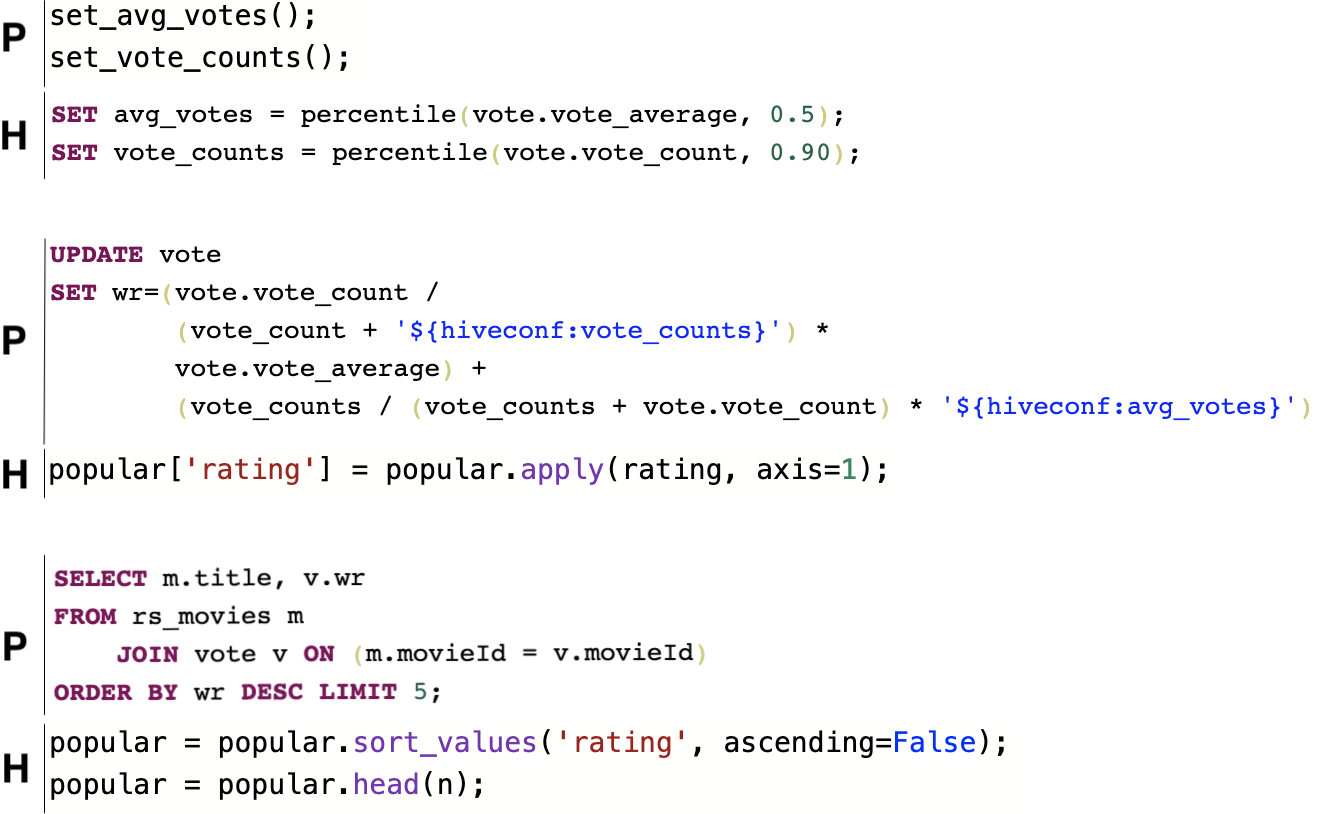
\includegraphics[width=1.0\textwidth]{images/python-hive}
  \caption{Comparaison entre le programme \texttt{Python} et \texttt{Hive}}
  \label{fig:python-hive}
\end{figure}

Cependant, il est possible de rencontrer quelques difficultés lorsque nous souhaitons réaliser un système plus complexe avec \texttt{Hive} comme un système basé sur le contenu du film. C'est pourquoi, nous avons décidé de réaliser cela en \texttt{Python}. Le but est de matcher les films ayant le plus de ressemblance  avec le film passé en paramètre. Le taux de ressemblance sera calculé à l'aide des descriptions, des tags, du titre des films, en utilisant la similarité cosinus $ cos \theta = \frac{A * B}{||A|| * ||B||} $ (fig.\ref{fig:python-cosine}). Puis il suffit de prendre les films pour lesquelles la valeur de la similarité cosinus est la plus élevé par rapport au film choisi pour avoir une bonne recommendation. A noter que nous utiliserons plutôt \texttt{linear\_kernel} lorsque nous utilisons l'objet \texttt{TfidfVectorizer} afin de gagner du temps.

\begin{figure}[H]
  \centering
  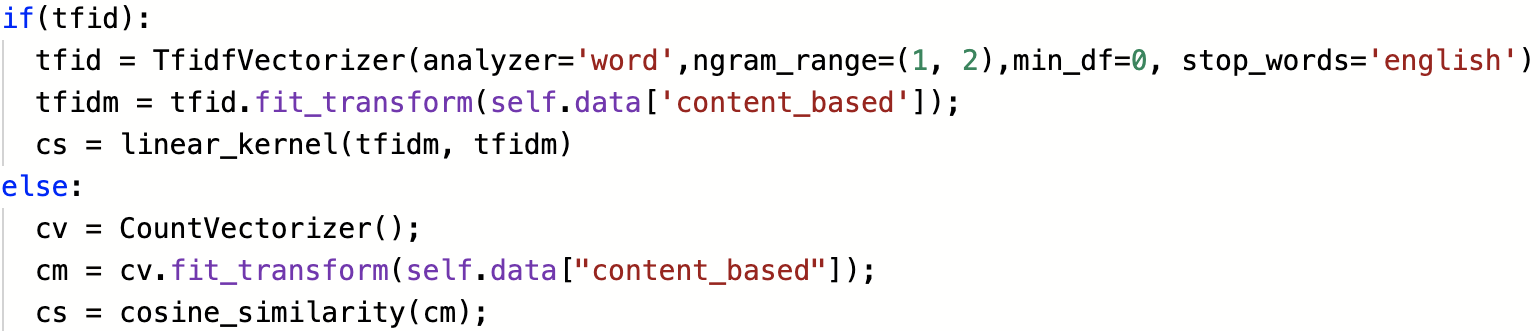
\includegraphics[width=1.0\textwidth]{images/python-cosine}
  \caption{L'utilisation de la similarité de cosinus pour calculer la similarité entre les films}
  \label{fig:python-cosine}
\end{figure}

\chapter{Conclusion}

Poru conclure, l'architecture distribuée représente une conception différente de la programmation dont nous avions pas l'habitude lors des années précédentes. Les services AWS représente de nombreux avantages: ils sont très maniables, faciles à utiliser, flexibles, très sécurisés les rendant ainsi fiables. Par ailleurs, ils peuvent êre exploités dans de nombreux cas, ce qui souligne un peu plus leur flexibilité. Et ce n'est d'ailleurs pas une surprise si ils sont utilisés par les plus grandes entreprises telles que Netflix, Expedia, Sysco ou encore Airbnb.

\bibliographystyle{alpha}
% \bibliography{memoire}
\end{document}
